\documentclass[english]{article}
\usepackage{comment}
\usepackage[letterpaper]{geometry}
\usepackage{tikz}
\usepackage{amsmath}
\usepackage{amsfonts}
\usepackage{amssymb}
\usepackage{float}
\usepackage{graphicx}
\usepackage{listings}
\usepackage{xcolor}

 
\definecolor{codegreen}{rgb}{0,0.6,0}
\definecolor{codegray}{rgb}{0.5,0.5,0.5}
\definecolor{codepurple}{rgb}{0.58,0,0.82}
\definecolor{backcolour}{rgb}{0.95,0.95,0.92}
 
\lstdefinestyle{mystyle}{
    backgroundcolor=\color{backcolour},   
    commentstyle=\color{codegreen},
    keywordstyle=\color{magenta},
    numberstyle=\tiny\color{codegray},
    stringstyle=\color{codepurple},
    basicstyle=\ttfamily\footnotesize,
    breakatwhitespace=false,         
    breaklines=true,                 
    captionpos=b,                    
    keepspaces=true,                 
    numbers=left,                    
    numbersep=5pt,                  
    showspaces=false,                
    showstringspaces=false,
    showtabs=false,                  
    tabsize=2
}
 
\lstset{style=mystyle}


\geometry{verbose,tmargin=1in,bmargin=1in,lmargin=1in,rmargin=1in}

\renewcommand{\u}{{\mathbf u}}
\newcommand{\x}{{\mathbf x}}
\newcommand{\R}{{\mathbb R}}


\title{CIS 520, Machine Learning, Fall 2020 \\ Homework 8\\
Due: Monday, December 7th, 11:59pm \\
Submit to Gradescope}
\date{}
\author{Yuezhong Chen; Sheil Sarda}


\begin{document}
\maketitle
\section{Reinforcement Learning}

\begin{enumerate}
\item 
Formulate an MDP for the \texttt{Chain} environment by specifying each component of the tuple $\mathcal{M} = \langle \mathcal{S},\mathcal{A},p,r,\gamma \rangle$. For the components $p$ and $r$, write down $p(s'|s,a)$ and $r(s,a,s')$ for each setting of $s,a,s'$ for which the probability/reward is non-zero:

The MDP formulation is as follows:
\begin{enumerate}
\item The set of states $\mathcal{S} = \{0,1,2,3,4\}$
\item The set of actions $\mathcal{A} = \{f,b\}$
\item In the states of 0 1 2 or 3, we have:\\

$p(0|i,f) = 0.1, p(0|i,b) = 0.9$ and $ p(i+1|i,f) = 0.9, p(i+1|i,b) = 0.1$\\
$r(i,f,0) = 2, 
r(i,f,i+1) = 0$ and $r(i,b,0) = 2, r(i,b,i+1) = 0$\\

When the state is 4, we have:\\

$p(0|4,f) = 0.1, p(0|4,b) = 0.9$ and $p(4|4,f) = 0.9, p(4|4,b) = 0.1$\\
$r(4,f,0) = 2, r(4,f,4) = 10$ and $r(4,b,0) = 2, r(4,b,4) = 10$
\end{enumerate}

\item
Find the optimal state-value function $V^*$, i.e.\ find the optimal value $V^*(s)$ for each state $s$:

$
V^* = 
\begin{bmatrix}
40.742& 45.525& 51.430& 58.720& 67.720
\end{bmatrix}
$\\

\item
Using your solution to the second part above, find an optimal deterministic policy $\pi^*$, i.e. find an optimal action $\pi^*(s)$ for each state $s$:

$ 
Q^* = 
\begin{bmatrix}
   40.742 & 38.898\\
   45.525 & 39.430\\
   51.430 & 40.086\\
   58.720 & 40.896\\
   67.720 & 41.896\\
\end{bmatrix}
$\\

The optimal policy is: 
$
\pi^{*} = 
\begin{bmatrix}
0&0&0&0&0
\end{bmatrix}
$\\
\end{enumerate}



\section{Reinforcement Learning: Q-Learning}

\subsection {``Traditional" Q-Learning} 

After running Q-learning using the parameters provided in the notebook, use the code provided to plot the \textbf{Average Reward, Success Rate, and Car Final Position vs Episodes}. Also give an image of your car reaching the flag in the final episode.
 

% avg reward
 \begin{figure}[H]
   \centering
     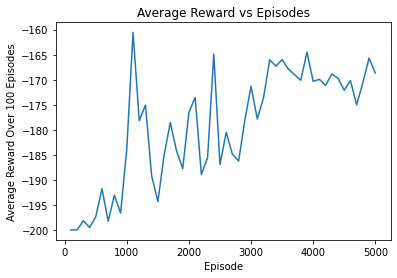
\includegraphics[scale=0.7]
     {templates/avg_reward1}
\end{figure}

% success rate
 \begin{figure}[H]
   \centering
     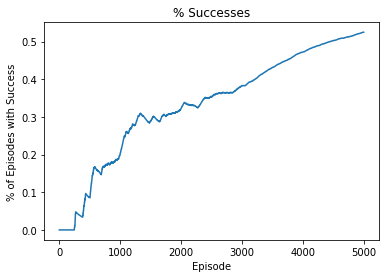
\includegraphics[scale=0.7]
     {templates/success1}
 \end{figure}

% car final position
 \begin{figure}[H]
   \centering
     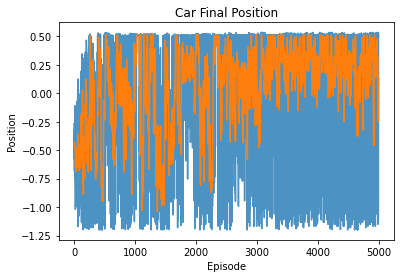
\includegraphics[scale=0.7]
     {templates/position1}
 \end{figure}

% car success image
 \begin{figure}[H]
   \centering
     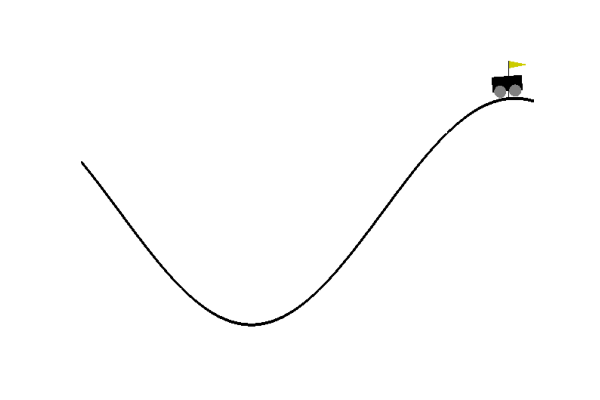
\includegraphics[scale=0.7]
     {templates/car1}
 \end{figure}

\subsection{Deep Q-Learning}

After running deep Q-learning using the parameters provided in the notebook, plot the \textbf{Success Rate, and Car Final Position vs Episodes}.

% success rate, deep
 \begin{figure}[H]
   \centering
     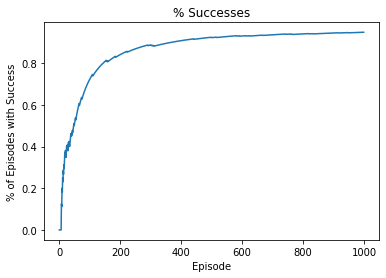
\includegraphics[scale=0.7]
     {templates/success2}
 \end{figure}

% car position, deep 
 \begin{figure}[H]
   \centering
     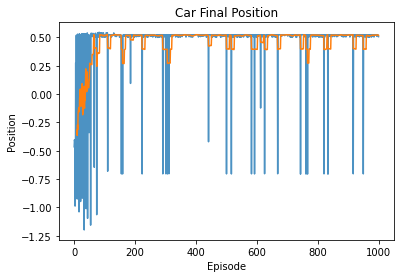
\includegraphics[scale=0.7]
     {templates/position2}
 \end{figure}

 \begin{figure}[H]
   \centering
     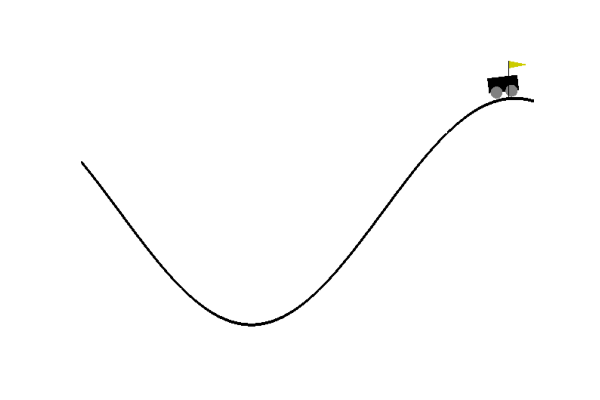
\includegraphics[scale=0.7]
     {templates/car2}
 \end{figure}

\subsection{Questions}
\begin{enumerate}
    \item As part of the Deep QLearning implementation, you implemented a $\mathsf{reward\_shaping}$ function to aid in the learning process. Compare this to the original reward structure in part 2.1 -- why do you think this modification of the reward is helpful?
    \newline
	Description of the reward shaping function: the reward is always 0.5 + the position of the car in the next state, and if the position of the car in the next state is greater than 05, add +1 on top of the computed reward. The original reward structure in 2.1 is un-shaped.
	\newline
	\newline
	In general, Reward shaping augments the natural reward signal in order to provide more frequent feedback on appropriate behaviors during the learning process. This modification of the reward is helpful because it gives the model more feedback during the training process which guides it towards successful outcomes earlier.

    \item Compare the \textbf{Success Rate} and \textbf{Car Final Position} plots between your two implementations. Which algorithm is learning a successful policy more quickly? Briefly comment on potential reasons for any differences in performance.
    \newline\newline
    Differences between the Deep Q-Learning and Standard Q-Learning models: 
    \begin{enumerate}
    \item Car reaches the final position (0.5) within 1000 iterations in the Deep Q-Learning model, whereas the standard Q-Learning model takes 5000 iterations.
    \item Success rate of the Deep Q-Learning model approaches 0.8 as an asymptote within the first 200 episodes, and then steadily makes progress towards a $100\%$ success rate.
    \item The Standard Q-Learning model follows a more linear trajectory in its success rate, and is only able to achieve a $50\%$ success rate at the end of 5000 iterations.
    \end{enumerate}
    
    Based on the above observations, we can conclude that the Deep Q-Learning model learns a successful policy quicker. The potential reasons for these performance differences include: (a) presence of a reward shaping function which provides the model with more feedback during the training process; (b) increased model complexity to better capture the complexity of the optimal policy.
    
\end{enumerate}

\section{Autoencoders}

\subsection{Part 1: Constructing the Autoencoder} 
    
The training curve is given below:


% Training curve
 \begin{figure}[H]
   \centering
     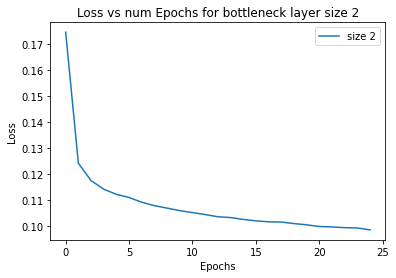
\includegraphics[scale=0.8]{templates/ae_curve1}
 \end{figure}

The reconstructions of the last minibatch for epochs 0, 10, and 20 are:


% Epoch 0
 \begin{figure}[H]
   \centering
     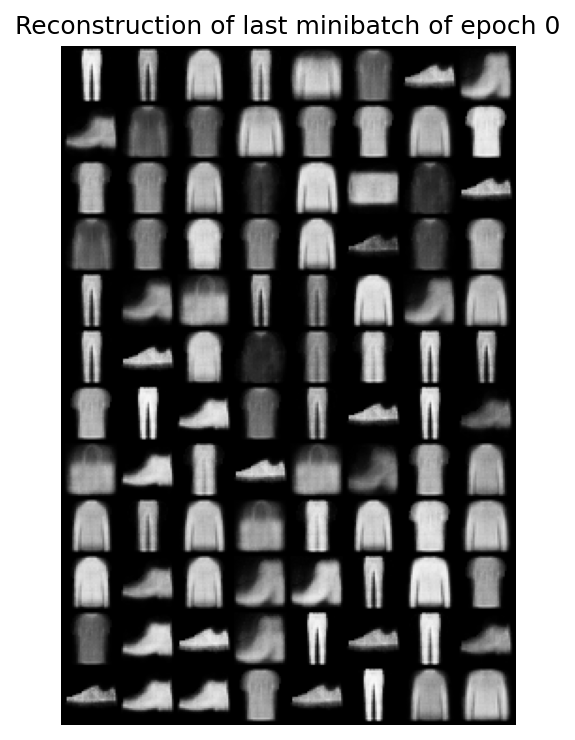
\includegraphics[scale=0.8]{templates/re0}
 \end{figure}

% Epoch 10
 \begin{figure}[H]
   \centering
     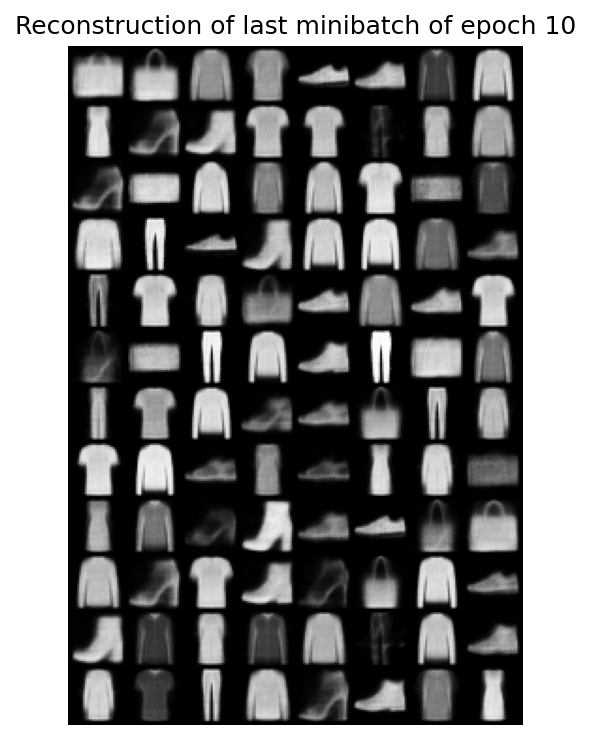
\includegraphics[scale=0.8]{templates/re10}
 \end{figure}

% Epoch 20
 \begin{figure}[H]
   \centering
     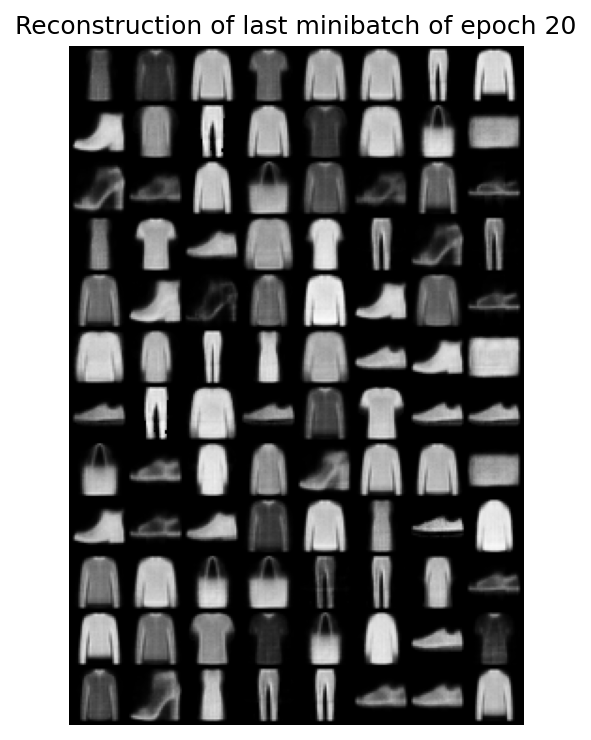
\includegraphics[scale=0.8]{templates/re20}
 \end{figure}


\subsection{Part 2: Latent Space Decomposition }
\begin{enumerate}
    \item Plot of the latent space of this autoencoder:
    
    Changed random seed to 40 to get a better latent space plot since the original one was a vertical line.
    % latent space plot
    \begin{figure}[H]
      \centering
         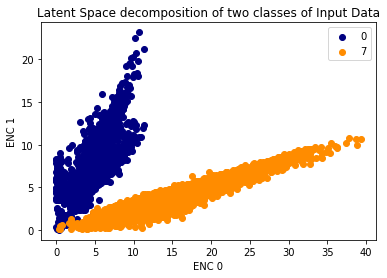
\includegraphics[scale=0.8]{templates/latent1}
    \end{figure}

    \item From the latent space plot, explain what the encoding has done to the inputs. How is this effect related to what PCA does? Why is this useful?
    \newline\newline
    The latent space is where encoded vectors lie. The encoder decreases the dimensionality of the input up to the latent space. PCA is looking for the best linear subspace of the initial space described by an orthogonal basis of new features such that the error of approximating the data by their projections on this subspace is as small as possible. 
	\newline \newline
	PCA and the Encoder are similar in that both are building new features using the features of the input dataset. The capability to compress data can be used for a variety of tasks such as removing noise / occlusions from images, developing lossy compression algorithms and machine translation.

\end{enumerate}

\subsection{Part 3: Reconstruction Error vs Bottleneck Layer} 
\begin{enumerate}
    \item Report the combined training curves (mean epoch loss vs epochs) for all the bottleneck layer sizes $[2,8,32,64]$. Also report the reconstructed images for Epoch 20 for each of the configurations.
    
    The training curves of all the configurations:

    % training curve plot
     \begin{figure}[H]
       \centering
         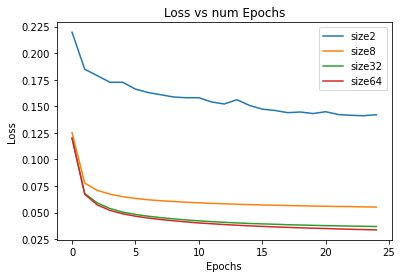
\includegraphics[scale=0.8]{templates/loss1}
     \end{figure}

The reconstructions for sizes $[2,8,32,64]$ for epoch 20 of the last minibatch:

% bottleneck 2
 \begin{figure}[H]
   \centering
     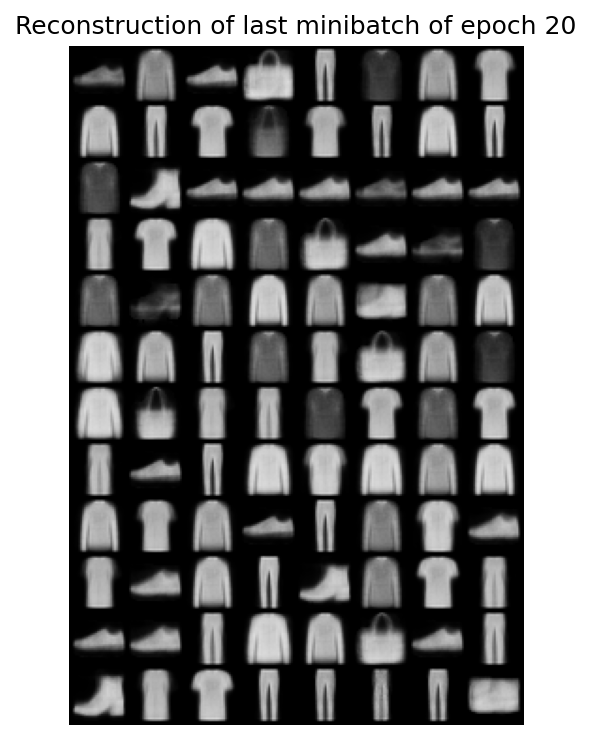
\includegraphics[scale=0.6]
     {templates/re20_2}
     \caption{Size 2}
 \end{figure}

% bottleneck 8
 \begin{figure}[H]
   \centering
     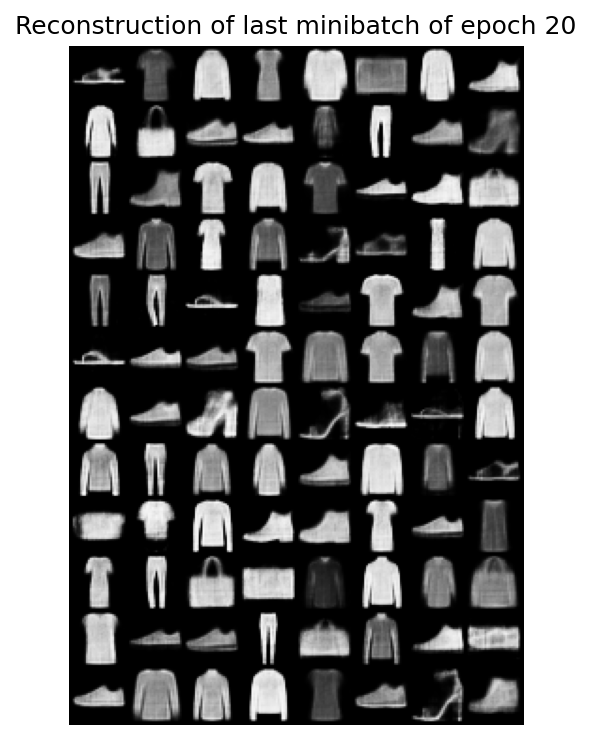
\includegraphics[scale=0.6]
     {templates/re20_8}
     \caption{Size 8}
 \end{figure}

% bottleneck 32
 \begin{figure}[H]
   \centering
     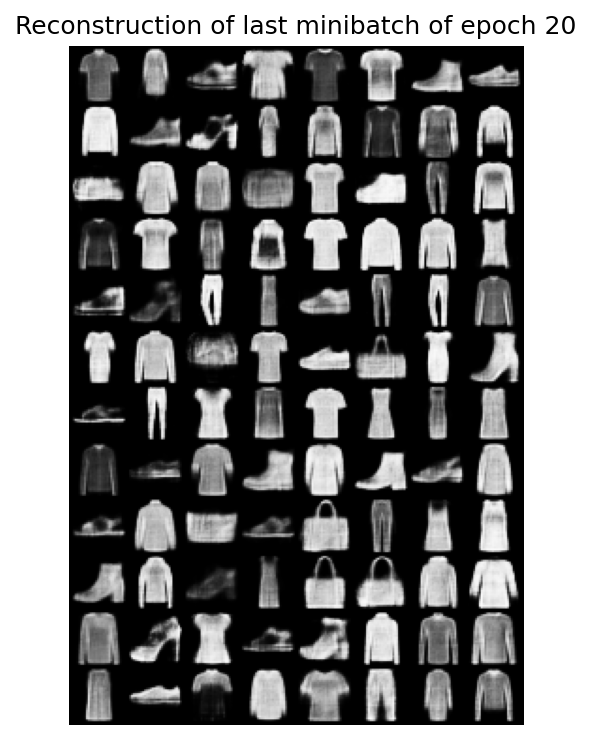
\includegraphics[scale=0.6]
     {templates/re20_32}
     \caption{Size 32}
 \end{figure}

% bottleneck 64
 \begin{figure}[H]
   \centering
     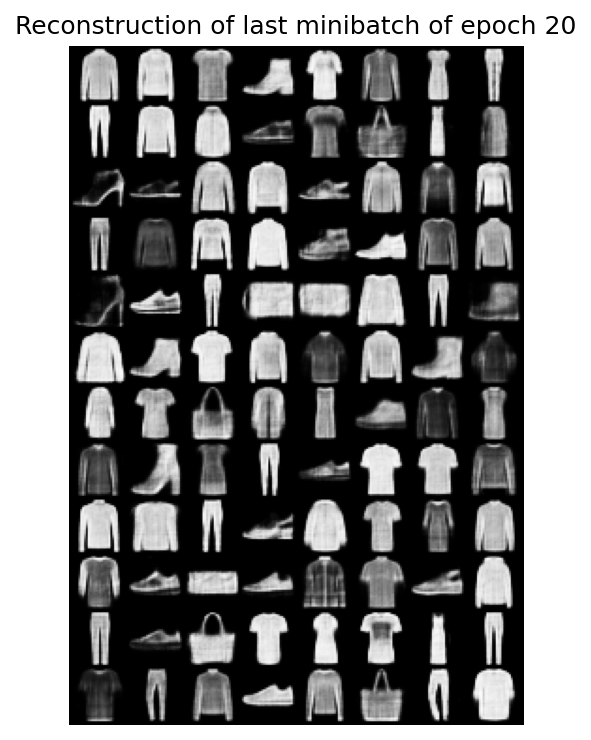
\includegraphics[scale=0.6]
     {templates/re20_64}
     \caption{Size 64}
 \end{figure}


\item 
The reconstruction error for images of class 0 as the bottleneck layer size increases:

% reconstruction vs size
 \begin{figure}[H]
   \centering
     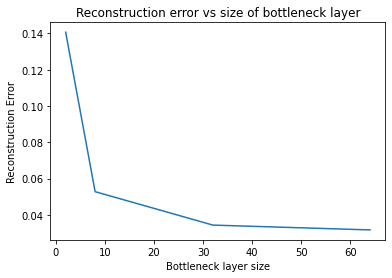
\includegraphics[scale=0.6]
     {templates/reconstruction1}
 \end{figure}

What are you observing? How does what you see relate to PCA? What does this tell you about how you can potentially work with a high-dimensional data-space?
\newline \newline
Observations based on how reconstruction error changes with bottleneck layer size, and similarities to PCA:
\begin{enumerate}
\item Inflection point at the bottleneck layer size of 32, indicating that 32 is the least number of dimensions required for optimally encoding the dataset.
\item Similar to how the PCA analysis helps determine the top $k$ features which account for most of the variance seen in the data, this analysis tells us that 32 features explain most of the variance in this dataset.
\end{enumerate}

Solutions for dealing with high-dimensional data spaces: (a) PCA to generate new features which are linear combinations of input features; (b) In a Vanilla Autoencoder, the latent space forms a bottleneck which forces the model to learn an effective compression of the data.

\end{enumerate}


\end{document}